\documentclass[reprint,amsmath,amssymb,aps,twoside]{revtex4-2}


\usepackage{graphicx}
\usepackage{amsmath,amssymb,amsfonts}
\usepackage{dcolumn}
\usepackage{bm}
\usepackage{siunitx}
\usepackage{tikz,pgfplots}
\sisetup{separate-uncertainty=true}
\usepackage[colorlinks,allcolors=blue]{hyperref}
\usepackage{cleveref}
\crefname{equation}{}{}
\crefname{figure}{Fig.}{Figs.}
\crefname{table}{Table}{Tables}
\usepackage{svg}
% set PDF metadata
\hypersetup{%
pdftitle={Investigating energy transformation: elastic potential energy to kinetic energy in a crossbow system},
pdfauthor={Dia Avalur, Srilekha Dantu, Jophy Lin, and Anika Tokala},
}
\usepackage{fancyhdr}
\pagestyle{fancy}
\fancyhf{}
\fancyhead[RE,RO]{J S\&E \textbf{1}, 63--66 (2025)}
\fancyhead[LO]{Avalur \emph{et al.}}
\fancyhead[LE]{Investigating energy transformation in a crossbow}
\fancyfoot[C]{\thepage}
\fancypagestyle{mytitlepage}{
\fancyhf{}
\fancyhead[C]{Journal of Science \& Engineering \textbf{1}, 63--66 (2025)}
\fancyfoot[C]{\thepage}
}




\begin{document}
\setcounter{page}{63}
\title{Investigating energy transformation: elastic potential energy to kinetic energy in a crossbow system}

\author{Dia Avalur}
\email{Contact author: 426davalur@frhsd.com}
\author{Srilekha Dantu}
\author{Jophy Lin}
\author{Anika Tokala}
\affiliation{Science \& Engineering Magnet Program, \href{https://manalapan.frhsd.com/}{Manalapan High School}, Englishtown, NJ 07726 USA}
\date{\today}

\begin{abstract}
This experiment investigated the transformation of elastic potential energy into kinetic energy during the launch of a dart from a crossbow. Using a spring scale, we measured the nonlinear force-displacement relationship of the crossbow string, yielding a maximum elastic potential energy of \qty{0.514}{\joule}. The dart was launched horizontally across a measured distance of \qty{4.40}{\meter}, and its flight time was recorded over three trials. Calculated kinetic energies varied between \qtyrange{0.1468}{0.2389}{\joule}, with an average of \qty{0.187\pm0.038}{\joule}, indicating that around 36.4\% of the potential energy was successfully converted into kinetic energy. The energy losses, attributed to factors such as air resistance, internal friction within the crossbow mechanism, and energy dissipation as heat and sound, highlight inefficiencies in the energy transfer process. Despite these losses, the results validate the principle of energy conservation. The alignment of force-displacement data with a quadratic regression model supports the accuracy of the measurements and the validity of numerical integration used to estimate potential energy. This study demonstrates the challenges of achieving ideal energy conservation in practical systems while emphasizing the robustness of conservation laws under non-ideal conditions.
\end{abstract}

\keywords{keywords here}

\maketitle\thispagestyle{mytitlepage}











\section{Introduction}
Energy plays a fundamental role in understanding motion and dynamics. According to the Law of Conservation of Energy, energy cannot be created or destroyed but only transformed from one form to another [1]. In this experiment, we investigated the transformation of elastic potential energy into kinetic energy during the launch of a dart from a crossbow. The elastic potential energy is stored in the string of the crossbow when it is pulled back, and this energy is released to propel the dart forward.
The elastic potential energy of the system \cite{young:2019:university,tipler,barrons} is given by:
\begin{equation}
U = \int F(x) dx
\label{eq:1}
\end{equation}
where $F(x)$ is the force exerted by the string as a function of its displacement $x$. Unlike ideal springs, where $F(x)=kx$ leads to a linear force-displacement relationship, our experimental results indicated a nonlinear, J-shaped curve for $F(x)$. This necessitated the use of numerical methods, specifically Riemann sums, to approximate the elastic potential energy stored in the string. Once the string is released, this potential energy is converted into the kinetic energy $KE$ \cite{young:2019:university,tipler,barrons} of the dart, given by:
\begin{equation}
KE = \frac{1}{2} m v^2
\label{eq:2}
\end{equation}
where $m$ is the mass of the dart (\qty{0.008}{\kilo\gram}) and $v$ is its velocity (\unit{\meter\per\second}). By measuring the force-displacement data, approximating the area under the curve using Riemann sums \cite{young:2019:university}, and calculating the velocity of the dart post-launch, we were able to analyze the energy conversion in the system.

The purpose of this lab was to calculate the potential energy stored in the crossbow string and compare it with the kinetic energy of the dart to assess the efficiency of energy transfer. We hypothesized that while the total energy should be conserved, discrepancies may arise due to external factors such as friction and air resistance, as well as limitations in our numerical approximation methods.











\section{Methods and materials}

\subsection{Key materials}
The materials used in this lab included a crossbow equipped with an elastic string, which was used to launch the dart and a dart of known mass [2] (both from Adventure Awaits, USA) which served as the projectile. A spring scale [3] (from EAI Education, Oakland, NJ) was utilized to measure the force exerted by the string as it was pulled back to various displacements. A measuring tape [4] (from DEWALT, Thailand) was used to measure the distance the string was pulled back from its equilibrium position and also the total distance traveled by the dart.

To measure the dart’s velocity immediately after launch, a stopwatch with a precision of 0.01 seconds (from Marathon Watch Company, Ontario, Canada) [5] was used to measure the time of flight for each trial. Additionally, clamps (from Harbor Freight Tools, Calabasas, CA) [6] were used to secure the crossbow to prevent movement during the experiment. Google Sheets was utilized to record force and displacement values, and Desmos’ graphing software was employed to create the force-displacement plot and perform computations.
\begin{figure}
\begin{center}
\includegraphics[width=\columnwidth]{Materials.png}
\end{center}
\caption{\label{fig:1} Lab materials. Collage of representative lab materials used during the experiment, including a crossbow, dart, spring scale, measuring tape, stopwatch, and clamps. Images sources from online platforms for illustrative purposes and cited.}
\end{figure}

\subsection{Measuring kinetic energy}
To measure the kinetic energy of the dart, a distance of 4.40 meters was marked on a table using the measuring tape. This distance extended from the crossbow’s position on the table to a vertical wall, ensuring that the dart would hit the wall and stop after being launched. The bottom of the crossbow was placed flat on the table, aligned with the measured distance, to ensure that the dart was launched horizontally without any tilt.

The dart was loaded onto the crossbow, and the string was pulled back to the desired displacement of \qty{0.10}{\meter}. The trigger was then released to launch the dart, allowing it to travel across the measured distance of \qty{4.40}{\meter} horizontally before striking the wall. This setup minimized external interference and ensured consistent motion in the horizontal direction.
For each launch, the time of flight was recorded in three separate trials to ensure consistency and accuracy in the results. The velocity of the dart was then determined using the equation \cite{young:2019:university}:
\begin{equation}
v = \dfrac{d}{t},
\label{eq:3}
\end{equation}
where $d=\qty{4.40}{\meter}$ the distance between the crossbow and the wall, and $t$ is the recorded time (in seconds) of flight for each trial. Using the calculated velocities, the kinetic energy  of the dart for each trial was determined using \cref{eq:2}. 

In addition to calculating the velocity and kinetic energy for each individual trial, the average time was calculated across all three trials. This average time was then used to compute an additional velocity and kinetic energy as supplementary data. The final results were presented as mean $\pm$ one standard deviation to account for variability in the measurements and provide extra supporting data.
\begin{figure}
\begin{center}
\includegraphics[width=\columnwidth]{setup.png}
\end{center}
\caption{\label{fig:2} Basic Sketch of Setup for Measuring the Kinetic Energy. Note: Only the gun for the crossbow is depicted here for readability and sketch is not to scale.}
\end{figure}

\subsection{Measuring potential energy}
To measure the potential energy stored in the crossbow string, we first secured the crossbow in place using clamps to prevent it from moving during the measurements. To simplify the process of measuring the force exerted by the string at different displacements, we removed the bow from the crossbow and laid it flat on the table. This setup ensured stability and accuracy during data collection. 
The spring scale was used to measure the force exerted by the string as it was pulled back incrementally. Using a ruler to measure displacement from the original position of the string, we pulled the string back in \qty{0.01}{\meter} increments. At each increment, the corresponding force was recorded using the scale. This process was repeated and stopped after recording the force at \qty{0.10}{\meter}, which is the distance the string had to be pulled back to launch the dart.

Once all the data points were collected, the force values were plotted against the displacement values to create a force- displacement graph. Using the resulting plot, we performed the appropriate regression method on the data to model the curve mathematically. To approximate the elastic potential energy stored in the string, we followed \cref{eq:1}
.
Since the relationship was nonlinear, we applied numerical approximation methods. The force-displacement curve was divided into small intervals of \qty{0.01}{\meter}, and the potential energy was estimated using the Riemann sum method\cite{young:2019:university}:
\begin{equation}
U = \sum F(x_i) \Delta x,
\label{eq:4}
\end{equation}
where $F(x_i)$ represents the force at each $\Delta x=\qty{0.01}{\meter}$ displacement interval. This method allowed us to calculate the approximate total potential energy stored in the string with high precision.









\section{Results}
\Cref{tab:1} presents the measured time, calculated velocity, and corresponding kinetic energy for three separate trials of the dart launch. The calculated velocity was derived from the measured time of flight using \cref{eq:3}, and the kinetic energy was determined using the dart's mass and velocity using \cref{eq:2}. The supplementary data calculated across the three trials were as follows: an average time of \qty{0.207\pm0.021}{\second}, an average velocity of \qty{21.51\pm2.20}{\meter\per\second}, and an average kinetic energy of \qty{0.187\pm0.038}{\joule}.
\begin{table}
\caption{\label{tab:1} Time, Velocity, and Kinetic Energy for Each Trial of the Dart Launch.}
\begin{center}
\includegraphics[width=\columnwidth]{table1.png}
\end{center}
\end{table}

\Cref{tab:2} presents the measured displacements of the crossbow string and the corresponding forces recorded using the spring scale. These measurements highlight the relationship between the displacement of the string and the force exerted on it.
\begin{table}
\caption{\label{tab:2} Displacement and Force Measurements for the Crossbow String.}
\begin{center}
\includegraphics[width=\columnwidth]{table2.png}
\end{center}
\end{table}

\Cref{fig:3} displays the force-displacement relationship for the crossbow string. The data points represent the force exerted by the string at various displacements. A quadratic regression was chosen because it best captures the observed nonlinear, J-shaped relationship between force and displacement, as determined experimentally. Among several models tested, the quadratic fit was found to provide the closest alignment with the measured data, minimizing error and producing the value 0.9718 as the coefficient of determination, which is indicative of a strong correlation. 
\begin{figure}
\begin{center}
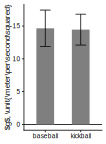
\includegraphics[width=\columnwidth]{fig3.png}
\end{center}
\caption{\label{fig:3} Force vs. Displacement Curve Representing the Nonlinear Relationship Between Force and Displacement for the Crossbow String.}
\end{figure}

Using \cref{eq:4} and the data from \cref{tab:2}, the elastic potential energy calculated is \qty{0.514}{\joule}.







\section{Discussion}

\subsection{Is energy conservation verified?}
\Cref{tab:1} shows that the calculated kinetic energies of the dart varied across the three trials, with values of \qtylist{0.1756;0.1468;0.2389}{\joule}, averaging \qty{0.187\pm0.038}{\joule}. When compared to the calculated elastic potential energy of \qty{0.514}{\joule}, it is evident that not all of the stored potential energy was converted into the dart’s kinetic energy. This discrepancy highlights energy losses during the energy transfer process, which are expected in real-world systems due to various inefficiencies.

\Cref{tab:2} and \cref{fig:3} illustrate the nonlinear force- displacement behavior of the crossbow string. The quadratic regression curve aligns closely with the measured data points, reflecting the J-shaped relationship between force and displacement. Using \cref{eq:4}, the total elastic potential energy stored in the string was calculated to be \qty{0.514}{\joule}. This value represents the maximum theoretical energy available for conversion into kinetic energy. However, only a portion of this energy was successfully transferred to the dart, as evidenced by the significantly lower kinetic energy values.

\subsection{Efficiency of energy conversion}
The significant difference between the elastic potential energy stored in the crossbow string (\qty{0.514}{\joule}) and the dart’s kinetic energy values, such as the average kinetic energy (\qty{0.187}{\joule}),  highlight the inefficiencies in the energy transfer process. Using the average kinetic energy value, approximately 63.6\% of the potential energy was lost, with only 36.4\% converted into kinetic energy. 

These inefficiencies can be attributed to multiple factors, including dissipation of energy as heat and sound during string release and vibration, air resistance acting on the dart, and friction within the crossbow mechanism. Hysteresis in the elastic string further reduced energy transfer, as internal damping prevented complete recovery of the stored energy. Additionally, recoil of the crossbow diverted energy away from the dart.

For comparison, modern compound bows have been noted to sometimes achieve efficiencies of 87\% to 89\% at transferring the archer’s input energy to the arrow [7]. This efficiency is significantly higher than the 36.4\% efficiency observed in this experiment, which emphasizes the impact of factors such as friction, material properties, and mechanical design on energy transfer. The lower efficiency of the crossbow used in this experiment is consistent with expectations for simpler mechanisms with higher friction and less optimized string materials. Bounding the frictional force specifically would require measuring the work done by the crossbow mechanism, which could be estimated in future experiments by analyzing recoil forces or deformation losses in the string. These comparisons provide a more comprehensive understanding of the energy losses observed in this system.

\subsection{Implications and validation of conservation laws}
Despite these inefficiencies, the results of this experiment validate the principle of energy conservation. When accounting for energy losses due to dissipation, friction, and air resistance, the total energy within the system aligns with theoretical expectations. The calculated elastic potential energy of the string (0.514 J) represents the maximum energy available for conversion, and the dart’s kinetic energy reflects the portion of energy successfully transferred. The alignment of the force-displacement data points with the quadratic regression curve in \cref{fig:3} further supports the accuracy of the measurements and reinforces the validity of the numerical methods used to estimate the potential energy. 

Beyond the experimental findings, this study has broader implications for improving the design and efficiency of energy-storing systems, such as toys, tools, and devices relying on elastic or mechanical energy.

The findings can inform better designs for crossbows and similar devices. For instance, enhancing string materials and reducing friction could optimize energy transfer, which might improve the performance of recreational crossbows or even historical reconstructions. Additionally, understanding energy conservation in a mechanical system like this can be applied to fields such as biomechanics, where similar principles govern the movement of elastic components in the human body. 

\subsection{Sources of experimental error}
Several experimental errors may have influenced the results, but these could be mitigated with improvements to the setup and methodology. Timing inaccuracies, resulting from the manual operation of the stopwatch, introduced variability in the measured flight times. Even with a precision of \qty{0.01}{\second}, human reaction time likely impacted the recorded data. This issue could be addressed by using an automated timing system, such as photogates, to measure the dart’s flight time more accurately [8]. 

Inconsistencies in the release mechanism of the crossbow string may have resulted in uneven application of force to the dart, further contributing to variations in the calculated velocities and kinetic energies. This could be addressed by having a mechanical release system to improve consistency [8].

The nonlinearity of the force-displacement curve is not inherently a source of error but requires more precise numerical treatment. The approximation method used to approximate the potential energy may have introduced errors, especially for intervals where the force increased rapidly. A more accurate approach would involve using the trapezoidal rule or Simpson’s rule for numerical integration, which better accounts for the curvature of the  graph. Alternatively, the fitted curve from the regression model could be used directly for integration, which would improve the accuracy of the potential energy calculation by eliminating the need for segmenting the data into discrete intervals.

External factors such as air resistance acting on the dart and internal friction within the crossbow mechanism also contributed to energy losses, reducing the overall efficiency of the system. These losses could be minimized by improving the crossbow design. For instance, using low-friction materials and lubricating moving parts would reduce internal energy dissipation. Additionally, replacing the current string with a material that has higher energy retention and lower hysteresis could reduce energy losses in the string itself. Finally, improving the aerodynamics of the dart would help minimize air resistance, which further increases the efficiency of energy transfer [8].





\section{Acknowledgements}
DA contributed by shooting the dart bullets across the measured surface, assisting with timing the dart’s flight, and helping write the lab report. JL helped to time the dart’s flight, record data, perform calculations, and contribute to the writing of the lab report. SD assisted in timing and visually identifying the moment the dart hit the surface to make sure of accurate measurements. AT helped by weighing the materials used in the experiment and shooting the darts during the trials.





%VI.   REFERENCES
%[1]
%	Young, H. D., & Freedman, R. A. (2019). University Physics with Modern Physics (15th ed.). Pearson Education.
%	[2]
%	Adventure Awaits. (n.d.). 2-Pack Handmade Wood Toy Crossbow Set - 12 Suction Darts - for Outdoor Play. Amazon. Retrieve from https://www.amazon.com/dp/B07Q4FC3H9
%	[3]
%	EAI Education. (n.d.). Spring Scale - White: 3kg/30 N. Retrieved from https://www.eaieducation.com/Product/530306
%	[4]
%	DEWALT. (n.d.). Atomic Compact Series 25 ft. Tape Measure. Amazon. Retrieved from https://www.amazon.com/dp/B0C1LM4
%5PQ
%	[5]
%	Marathon Watch Company. (n.d.). ADANAC 4000 Digital Stopwatch Timer. Retrieved from https://www.marathonwatch.co
%m/products/adanac-4000-digital-stopwatch-timer
%	[6]
%	Harbor Freight Tools. (n.d.). 6-Inch Industrial C-Clamp. Retrieved from https://www.harborfreight.com/6-inch-industrial-c-clamp-37
%850.html
%	[7]
%	Hass, Corey. (2017.). How Compound Bows Work. Outside Online. Retrieved from https://www.outsideonline.com/outdoor-g
%ear/tools/how-compound-bows-work/
%	[8]
%	Taylor, J. R. (1997). An Introduction to Error Analysis: The Study of Uncertainties in Physical Measurements (2nd ed.). University Science Books.
%\bibliography{avalur.bib}
\end{document}
